\documentclass[11pt]{article}
\usepackage[utf8]{inputenc} % standard input encoding
\usepackage[T1]{fontenc} % standard modern font encoding
\usepackage{lmodern} % use Latin Modern font (it has vectorized special characters = better copying od searching in pdfs)
\usepackage[czech]{babel}
\usepackage[a4paper]{geometry} % margin adjustment
\usepackage[pdfusetitle]{hyperref} % metadata, content in pdf, hyperlinks
\usepackage{caption} % hyperlinks navigate to the top of the images
\usepackage{easyReview}
\usepackage{array}
\usepackage{bm}

\usepackage{graphicx}
\graphicspath{ {./images/} }

% bibliography
\usepackage[backend=bibtex]{biblatex}
\addbibresource{bibliography.bib}

\def\MainTitle{Automatická detekce ischemické léze z MR obrazových dat u cévní mozkové příhody}
\def\Subtitle{Diplomový projekt}
\date{\large \hfill \today}

\hypersetup{pdftitle={\MainTitle}} % add main title to the pdf metadata
\title{
	\ifdefined\Subtitle \large \Subtitle \\[1em] \fi
	\LARGE \textbf{\MainTitle} \\[2em]
	\begin{large}
	\begin{minipage}{3cm}
		\textbf{Autor:}\\
		Jakub Šmíd
	\end{minipage}
	\hfill
	\begin{minipage}{6cm}
		\textbf{Vedoucí:}\\
		prof. MUDr. Jakub Otáhal, Ph.D. \\
		Ing. David Kala
	\end{minipage}
	\end{large}
}

\begin{document}
\maketitle

\section{Popis projektu}
Cévní mozková příhoda (mrtvice) je jedním z nejčastějších onemocnění a příčin úmrtí celosvětově. Zásadní krok při jejím vyšetření je segmentace poškozené tkáně na obrazech z magnetické resonance. V současné klinické praxi se segmentace provádí manuálním obkreslováním a kvůli tomu je velmi časově náročná a výsledky podléhají značné subjektivitě. Cílem této práce je celý proces zrychlit přidáním prvků automatické segmentace obrazu.
Práce bude probíhat v úzké spolupráci s Fakultní nemocnicí v Motole a neurovědci z EpiReC zabývající se dlouhodobě problematikou cévní mozkové příhody a souvisejících onemocnění.

Téma propojuje technické znalosti (zpracování obrazu, návrh algoritmů) s lékařským prostředím neurověd.

\section{Segmentace}
\section{Evaluační metriky}
Před tím, než se začneme věnovat publikacím a aktuálnímu stavu poznání, je nutné uvést metriky, na základě kterých budeme moci vyhodnotit úspěšnost segmentačních algoritmů. Díky uvedeným metrikám je možné srovnat kvalitu dvou segmentací stejného vzoru - typicky segmentaci experta (radiologa) a automatickou segmentaci.

Pro porovnání dvou segmentací jsou používány následující míry: dice similarity coefficient, average symetric surface distance. Pro vyhodnocení \alert{over- a under-segmentation} se používají metriky známé pod pojmy precision a recall. \cite{Maier2016, Ito2018}
\subsection{Dice similarity coefficient}
Dice similarity coefficient dále označovaný jako DC je mírou přesnosti segmentace.
\begin{equation}
	\label{DC}
	DC = 2 \frac{|A \cap B|}{|A|+|B|}
\end{equation}
Vztah pro výpočet DC je dán rovnicí \ref{DC}, kde A a B jsou dvě poměřované segmentace. DC koeficient nabývá hodnot mezi 0 a 1 a popisuje překryv mezi jednotlivými segmentacemi. Porovnávání dvou různých DC je citlivé na velikost segmentovaného prostoru (léze). DC dosahuje vyšších hodnot u segmentací s větším objemem.

\subsection{Average symetric surface distance}
Pro výpočet average symetric surface distance (dále ASSD) je nutné nejprve vypočítat tzv. average surface distance (ASD).
\begin{equation}
	\label{ASD}
	ASD(A_S, B_S) = \frac{\sum_{a \in A_S} \min_{b \in B_S} d(a,b)}{|A_S|}
\end{equation}
ASD je definován vztahem \ref{ASD}, kde $d(a,b)$ je 3D matice obsahující Euklidovské vzdálenosti mezi segmentacemi A a B. Potom ASSD se vypočítá podle vztahu \ref{ASSD}.
\begin{equation}
	\label{ASSD}
	ASSD(A_S, B_S) = \frac{ASD(A, B) + ASD(B, A)}{2}
\end{equation}
ASSD je tedy míra vyjadřující průměrnou vzdálenost všech Euklidovských vzdáleností mezi jednotlivými osegmentovanými objemy. Standardně se uvádí v milimetrech a nižší ASSD znamená lepší úspěšnost segmentace - resp. segmentace jsou si vzájemně podobnější.

\subsection{Hausdorffská vzdálenost}
Hausdorffská vzdálenost (Hausdorff's distance, dále HD) je míra vyjadřující maximální vzdálenost mezi odpovídajícími body, které tvoří hranici jednotlivých segmentací. Tato míra je tedy citlivá na \alert{outliery}.
\begin{equation}
	\label{HD}
	HD(A_S, B_S) = \max \{\max_{a \in A_S}\min_{b \in B_S} d(a,b), \max_{b \in B_S}\min_{a \in A_S} d(b,a)\}
\end{equation}
HD je definována vztahem \ref{HD}, a podobně jako ASSD se i HD běžně uvádí v milimetrech a nižší vzdálenost HD znamená lepší úspěšnost.

\subsection{Precision}
\subsection{Recall}

\section{Doporučená literatura}
\subsection{ISLES 2015}
Benchmarková studie \cite{Maier2016} zmiňuje problém komparability jednotlivých algoritmů pro segmentaci ischemické léze z důvodu různorodosti používaných datasetů a evaluačním procesům. Tento problém se autoři rozhodli vyřešit na soutěži Ischemic Stroke Lesion Segmentation challenge (ISLES) v roce 2015. Článek navrhuje evaluační proces, zmiňuje veřejně dostupné datasety a kromě toho nabízí srovnání výsledků z ISLES, které se zúčastnilo 16 vědeckých týmů.

Soutěž byla rozdělena na dvě kategorie. První z nich řešila Stroke Perfusion Estimation (SPES) - řešitelé se zaměřili na interpretaci obrazů akutní fáze mozkové mrtvice (0-24 hodin). Druhou kategorií byla Sub-acute Ischemic Stroke lesion Segmentation (SISS), kde bylo cílem analyzovat obrazy z pozdějších fází mrtvice (24 hodin - 2 týdny).

Data pro SISS byla nasbírána ze dvou zdravotnických zařízení, byla pořízena na stroji s magnetickým polem 3 T. Celkem bylo do datasetu zahrnuto 64 pacientů. Snímky pacientů, kteří byli zařazeni do datasetu, musely obsahovat alespoň sekvence T1-vážený, T2-vážený, DWI (b = 1000) a FLAIR. Segmentace pro trénink modelů byla provedena pouze na sekvenci FLAIR, jelikož tato sekvence vykazuje nejnižší variabilitu při segmentování mezi různými experty. Zbylá data poskytovala pouze podpůrnou informaci. Snímky pacientů byly rozděleny následovně: 28 pacientů pro trénink a 36 pro testování.

Výsledky kategorie SISS jsou zobrazeny v tabulce \ref{tbl-siss_results}. Jelikož dataset byl anotován dvakrát - podruhé jiným expertem, obsahuje tabulka výsledků na posledním řádku porovnání těchto dvou segmentací. Vizualizace výsledků je na obrázku \ref{img-isles2015}. Je nutné zmínit, že žádný z navržených algoritmů nedosáhl kladného Dice koeficientu u všech 36 pacientů z testovací sady. To znamená, že u některých snímků nedošlo k překryvu segmentací mezi expertem a algoritmem.

\begin{figure}[htp]
	\centering
	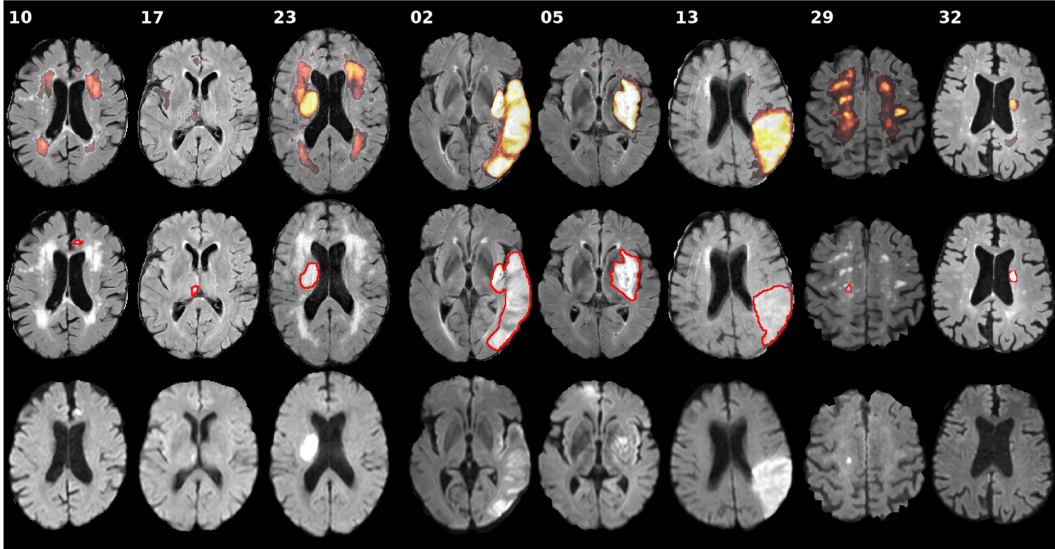
\includegraphics[width=\textwidth]{isles2015}
	\caption{Příklady snímků a výsledků z SISS. První řádek zobrazuje distribuci segmentace navržených metod na sekvenci FLAIR, druhý řádek zobrazuje stejný snímek segmentovaný expertem a na třetím řádku se nachází odpovídající DWI sekvence.}
	\label{img-isles2015}
\end{figure}

\begin{table}[htp]
	\centering
	\begin{tabular}{cllll}
		\textbf{Method} & \multicolumn{1}{c}{\textbf{Cases}} & \multicolumn{1}{c}{\textbf{ASSD (mm)}} & \multicolumn{1}{c}{\textbf{DC {[}0,1{]}}} & \multicolumn{1}{c}{\textbf{HD (mm)}} \\ \hline
		UK-Imp2         & 34/36                              & 05.96 $\pm$ 09.38                         & 0.59 $\pm$ 0.31                              & 37.88 $\pm$ 30.06                       \\ \hline
		CN-Neu          & 32/36                              & 03.27 $\pm$ 03.62                         & 0.55 $\pm$ 0.30                              & 19.78 $\pm$ 15.65                       \\ \hline
		FI-Hus          & 31/36                              & 08.05 $\pm$ 09.57                         & 0.47 $\pm$ 0.32                              & 40.23 $\pm$ 33.17                       \\ \hline
		US-Odu          & 33/36                              & 06.24 $\pm$ 05.21                         & 0.43 $\pm$ 0.27                              & 41.76 $\pm$ 25.11                       \\ \hline
		BE-Kul2         & 33/36                              & 11.27 $\pm$ 10.17                         & 0.43 $\pm$ 0.30                              & 60.79 $\pm$ 31.14                       \\ \hline
		DE-UzL          & 31/36                              & 10.21 $\pm$ 09.44                         & 0.42 $\pm$ 0.33                              & 49.17 $\pm$ 29.6                        \\ \hline
		US-Jhu          & 33/36                              & 11.54 $\pm$ 11.14                         & 0.42 $\pm$ 0.32                              & 62.43 $\pm$ 28.64                       \\ \hline
		UK-Imp1         & 34/36                              & 11.71 $\pm$ 10.12                         & 0.44 $\pm$ 0.30                              & 70.61 $\pm$ 24.59                       \\ \hline
		CA-USher        & 27/36                              & 09.25 $\pm$ 09.79                         & 0.35 $\pm$ 0.32                              & 44.91 $\pm$ 32.53                       \\ \hline
		BE-Kull         & 30/36                              & 12.24 $\pm$ 13.49                         & 0.37 $\pm$ 0.33                              & 58.65 $\pm$ 29.99                       \\ \hline
		CA-McGill       & 31/36                              & 11.04 $\pm$ 13.68                         & 0.32 $\pm$ 0.26                              & 40.42 $\pm$ 26.98                       \\ \hline
		SE-Cth          & 30/36                              & 10.00 $\pm$ 06.61                         & 0.38 $\pm$ 0.28                              & 72.16 $\pm$ 17.32                       \\ \hline
		DE-Dkfz         & 35/36                              & 14.20 $\pm$ 10.41                         & 0.33 $\pm$ 0.28                              & 77.95 $\pm$ 22.13                       \\ \hline
		TW-Ntust        & 15/36                              & 07.59 $\pm$ 06.24                         & 0.16 $\pm$ 0.26                              & 38.54 $\pm$ 20.36                       \\ \hline
		Inter-observer  & 34/36                              & 02.02 $\pm$ 02.17                         & 0.70 $\pm$ 0.20                              & 15.46 $\pm$ 13.56                       \\ \hline
	\end{tabular}
	\caption{Výsledky jednotlivých týmů na ISLES 2015 pro SISS.}
	\label{tbl-siss_results}
\end{table}

Autoři článku uvádí, že nejsou schopni jasně rozhodnout o rozdílech ve výkonnosti navržených metod - a to ani v typech jednotlivých přístupů (deep nebo klasický). Dvě nejlépe hodnocené metody, vykazovaly statisticky stejnou přesnost: metoda UK-Imp2 (později pojmenovaná DeepMedic) používala hluboké učení - konkrétně \alert{neuronové konvoluční sítě}, metoda CN-Neu byla založená na fuzzy c-means. Třetí nejlepší metoda byla založená na náhodných lesech (\alert{Random Forest}). Přesto nelze říci, že by nějaká z nich pracovala výrazně lépe. Autoři zmiňují, že klíčem k úspěchu je spíše odladění hyperparametrů modelu a jeho adaptace. Nejlepší tři řešení využívaly kombinaci dvou různých algoritmů, aby vykompenzovaly slabá místa každého z nich.

Metody soutěžících byly rovněž otestovány na datech z jiných zdravotnických center. Zajímavým výstupem soutěže je zjištění, že ani jeden z algoritmů nebyl schopen dobře fungovat na cizích datech. Přestože metody vykazovaly dobrou generalizaci na testovacích datech pořízených ze stejného datacentra jako data trénovací. Hypotéza, proč nedocházelo k \alert{overfittingu} je, že kvůli vysokému inter-rater Dice koeficientu (tzn. variabilitě segmentací napříč experty) nebyly schopny se ani modely přeučit na trénovací data.

Automatická segmentace obecně fungovala dobře na velkých lézích se silným FLAIR signálem, naopak byl problém v segmentaci malých lézí se slabým FLAIR signálem. Dalším problémem byla segmentace WMH (\alert{white matter hyperintensity}), místo ischemické léze. Toto zjištění je podle autorů překvapující, protože WMH není rozpoznatelná na DWI sekvenci (na rozdíl od léze), jelikož má stejnou intenzitu jako okolní tkáň - není viditelná.

Článek hodnotí SISS jako velmi obtížnou úlohu - nejen na základě přesnosti navržených metod, ale i na velkém rozptylu DC napříč experty. Podle autorů by kliničtí výzkumníci neměli očekávat spolehlivé a plně automatické řešení v blízké budoucnosti, jelikož je úloha příliš složitá. Automatické segmentační algoritmy by měly sloužit spíše jako podpůrný nástroj pro radiology.

Soutěž ukázala, že aktuální stav automatické segmentace sub-akutní léze postrádá jak přesnost, tak robustnost, která je potřebná pro reálné nasazení. Dalším zjištěním bylo, že žádný z algoritmů nefungoval významně lépe proti ostatním.

Pro budoucí výzkum autoři doporučují kombinovat různé algoritmy pro vylepšení segmentace. Evaluace by nikdy neměla být prováděna pouze na privátním datasetu a měl by být kladen důraz na adaptaci algoritmů na data z jiných center.

\subsubsection{DeepMedic \cite{uk-imp2}}
Segmentační metoda je založená na 3D konvoluční neuronové síti (CNN) s 11 vrstvami. Dataset, na kterém autoři trénovali neuronovou síť byl augmentován zrcadlením snímků přes sagitální rovinu. Před samotnou segmentací je 3D snímek rozdělen do několika batchů, díky tomu autoři zmenší počet trénovaných parametrů sítě. Následně vstupuje daný 3D batch do dvoucestné konvoluční sítě - do první cesty v plném rozlišení a do druhé cesty v nízkém rozlišení. Poté jsou obě cesty spojeny a příznaky vstupují do fully connected vrstev (FC). Autoři používají malá konvoluční jádra a tím snižují nároky na GPU paměť. Přestože architektura pracuje na 3D snímcích, lze ji natrénovat na grafické kartě, která má pouze 3 GB paměti.

\subsubsection{CN-Neu (Chaolu Feng) \cite{cn-neu}}
Tato metoda nepotřebuje žádná trénovací data, jelikož k segmentaci používá fuzzy c-means. Pro každou vstupní sekvenci proběhne segmentace na bílou hmotu, šedou hmotu mozkovou, mozkomíšní mok a lézi. Za lézi je následně určen ten voxel, který byl označen za lézi ve FLAIR sekvenci a zároveň alespoň v nějaké další sekvenci. Nakonec autoři upraví hranice léze podle vlastního algoritmu, jež je matematicky formulován v citovaném článku.

\subsection{Segmentace chronické mrtvice z T1-váženého obrazu}
Jelikož většina rehabilitačních metod po mozkové mrtvici závisí na T1-váženém obrazu, rozhodli se autoři článku \cite{Ito2018} provést srovnání jedné semi-automatické a tří plně automatických segmentačních algoritmů lézí z T1-vážených obrazů. Motivací bylo jejich systematické otestování na velkém datasetu.

Chronickou fázi autoři definují jako časové období od několika týdnů po roky od mozkové příhody. Pro rehabilitační účely se z časových a finančních důvodů pacient typicky snímkuje pouze sekvencí T1-w ve vysokém rozlišení. Tato sekvence je zároveň citlivá na zobrazení nekrózy vzniklé od 2 týdnů po příhodě, proto je vhodná k detekci chronických lézí.

Semiautomatická metoda \textbf{Clusterize} byla původně vyvinutá pro sledování ztráty myelinu při leukodystrofii. Ukázalo se však, že metoda založená na analýze T2-w, funguje i pro segmentaci akutní a chronické mrtvice z T1-w. \cite{DEHAAN201569} Clusterize nejprve vyhledává lokální maxima intenzity voxelů na každém snímku. Následně přiřadí zbylé voxely podle jejich intenzity do klastrů identifikovaných podle vyhledaných maxim. Poté musí člověk manuálně vybrat v každém řezu požadovaný klastr a případně udělat korekci masky.

První plně automatickou metodou zkoumanou v článku \cite{Ito2018} je \textbf{Automated Lesion Identification (ALI)} \cite{ali}, která je založená na detekci outlierů. Outliery jsou získány fuzzy clusteringem (c-means) pravděpodobnostních map bílé a šedé hmoty mozkové pacienta a kontrolních map. Kontrolní mapy jsou vygenerované ze zdravé tkáně - proto je třeba vlastnit dataset obsahující zdravé MRI snímky. Segmentace tkání je realizována iterativně softwarem \alert{SPM}, autoři uvádí novou třídu tkáně nazvanou "extra", která je průměrem již osegmentované pravděpodobnostní mapy bílé hmoty a mozkomíšního moku. Tato nová třída tkáně vstupuje do další iterace SPM segmentace a napomáhá ke správné segmentaci bílé a šedé hmoty. Po poslední iteraci se mapy bílé a šedé hmoty mozkové gaussovsky vyhladí a na takovýchto datech se hledají výše popsaným způsobem outliery.

Druhá automatická metoda \cite{gnb} implementuje \alert{\textbf{Gaussovský naivní Bayes}} klasifikátor. Pomocí softwaru SPM jsou získány pravděpodobnostní mapy tkání (bílé hmoty, šedé hmoty a mozkomíšního moku). Tyto mapy jsou společně s originálním T1-w obrazem transformovány do prostoru atlasu Montreal Neurological Institute a vyhlazeny gaussovským kernelem. Poté jsou z pravděpodobnostních map vygenerovány dvě mapy příznaků zobrazené na obrázku \ref{img-gnb_features}. Pro vygenerování map je potřebná znalost, v jaké hemisféře se léze nachází. První příznaková mapa $F_1$ obsahuje informaci o chybějící tkáni, která odpovídá jádru chronické léze. Vztah pro výpočet mapy je odvozen ze znalosti, že SPM segmentuje chronickou lézi spíše jako mozkomíšní mok, než jako bílou/šedou hmotu mozkovou. Druhá příznaková mapa $F_2$ obsahuje informaci o abnormální tkáni a vztah vychází z faktu, že tato tkáň má podobné hodnoty T1-w jako šedá hmota. Mapy příznaků jsou následně použity pro natrénování naivního Bayes klasifikátoru. Bylo použito 30 snímků pacientů a trénování probíhalo metodou, kdy jeden z pacientů sloužil jako validační data a zbytek jako trénovací, v další učící iteraci byl vybrán jiný pacient jako validační a zbylé snímky pacientů sloužily opět jako trénovací data. Tato metoda se v odborně označuje jako leave-one-case-out cross validation. Pro získání segmentace byl výstup thresholdován.
\begin{figure}[htp]
	\centering
	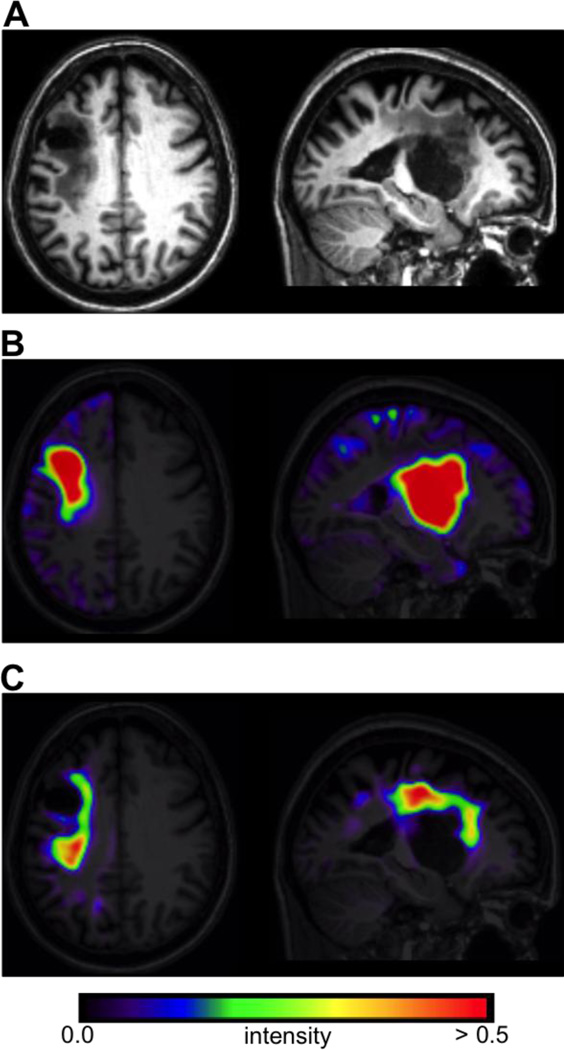
\includegraphics[width=6cm]{gnb_features}
	\caption{A zobrazuje T1-w obraz jednoho z pacientů. B znázorňuje příznaky $F_1$, tedy chybějící tkáň pro stejného pacienta. C znázorňuje příznaky $F_2$, tedy abnormální tkáň pro stejného pacienta.}
	\label{img-gnb_features}
\end{figure}

Poslední zkoumanou metodou byla \textbf{LINDA} \cite{LINDA}, kterou tvoří série \alert{náhodných lesů}. Metoda se skládá ze tří náhodných lesů, kdy každý z nich je navržen na jiné rozlišení dat. Vstupní MRI obraz je nejprve registrovaný na univerzální šablonu mozku, následně jsou z něj vypočítány různé \alert{příznaky} (např. odchylka od atlasu, levo-pravá asymetrie, gradient). Získané příznaky jsou poté převedeny do nižšího rozlišení. Každý řádek matice dat, která je použitá pro trénink a predikci v náhodném lese, se skládá z příznaků pro daný \alert{voxel} a jeho okolí. Rozhodování v lese tedy závisí nejen na příznacích jednoho voxelu, ale i na jeho okolí. Výstupem rozhodování v náhodném lese je \alert{mapa posteriorní pravděpodobnosti}, která je předána do další iterace, kde se používá již větší rozlišení příznaků, které opět vstupují do náhodného lesa. Výstupní pravděpodobnostní mapa ze třetího náhodného lesa se převede na segmentaci zdravá/postižená tkáň. Pro použití této metody je nutné, aby se léze nacházela v levé hemisféře, proto autoři srovnávací studie zrcadlově obracely obrazy, na kterých se léze nacházela v pravé hemisféře.

Tato srovnávací studie používala již předučené modely, které dodali autoři srovnávaných metod. Validace proběhla na \alert{datasetu ATLAS}, z něhož bylo použito 181 T1-w snímků pacientů. Každý ze snímků byl anotován jednou osobou ze skupiny jedenácti lidí, kteří byli předem podrobeni tréninku.

Z porovnání metod mezi sebou byly odstraněny ty snímky, kde některá z metod nedokázala osegmentovat žádný voxel, přestože na snímku byla léze. Také byly odstraněny snímky, u kterých všechny tři metody osegmentovaly voxely tak, že nenastal průnik se segmentací experta (misclassified). Selhání jednotlivých metod je možné vidět v tabulce \ref{tbl-t1w-misclassified}.
\begin{table}[htp]
	\centering
	\begin{tabular}{lp{5cm}p{5cm}}
		& \textbf{prázdná segmentace} & \textbf{prázdný průnik se segmentací experta} \\ \hline
		ALI         & 24                          & 28                                            \\ \hline
		naive Bayes & 0                           & 39                                            \\ \hline
		LINDA       & 23                          & 45                                            \\ \hline
		& 8 překryvů pro LINDA a ALI  & 10 překryvů mezi všemi metodami               \\ \hline
	\end{tabular}
	\caption{Počty pacientů (z celkových 181), u kterých segmentace kompletně selhala.}
	\label{tbl-t1w-misclassified}
\end{table}
\begin{table}[htp]
	\centering
	\begin{tabular}{ccccc}
		\textbf{Method} & \textbf{Cases} & \textbf{DC} & \textbf{ASSD (mm)} & \textbf{HD (mm)} \\ \hline
		Clusterize      & 152            & 0.23 ± 0.19 & 13.59 ± 5.85       & 75.00 ± 22.88    \\ \hline
		ALI             & 132            & 0.36 ± 0.25 & 14.38 ± 13.53      & 61.55 ± 28.84    \\ \hline
		naive Bayes     & 132            & 0.39 ± 0.23 & 10.49 ± 6.25       & 58.00 ± 19.73    \\ \hline
		LINDA           & 132            & 0.45 ± 0.31 & 12.68 ± 16.49      & 42.07 ± 24.38    \\ \hline
		inter-rater     & 5              & 0.75 ± 0.18 &                    &                  \\ \hline
	\end{tabular}
	\caption{Porovnání Dice coefficientu (DC), average symetric surface distance (ASSD) a Hausdorffské vzdálenosti (HD). Z evaluačního datasetu byly odstraněny některé snímky, u kterých segmentační metody nefungovaly. Poslední řádek zobrazuje DC při porovnání segmentací mezi dvěma experty u vybraných pěti pacientů.}
	\label{tbl-t1w-results}
\end{table}

Výsledky studie ukázaly, že všechny čtyři metody vykazují vysokou chybovost. Konkrétní hodnoty evaluace jsou k dispozici v tabulce \ref{tbl-t1w-results}. Úspěšnost segmentace léze je velmi závislá na velikosti a lokalizaci léze. Autoři článku analyzovaly případy pacientů, u kterých jednotlivé metody pracovaly velmi špatně (DC při evaluaci pod prvním kvartilem) nebo naopak velmi dobře (DC nad třetím kvartilem). Byly vytvořeny kategorie polohy léze a velikosti. Velikosti (malá, střední, velká) byly získány rozdělením celého datasetu na třetiny. Výsledky analýzy jsou uvedeny v tabulce \ref{tbl-t1w-size}, ze které vyplývá, že problém nastal nejčastěji při segmentaci malé léze v subkortikální oblasti, v mozkovém kmeni nebo v mozečku. Naopak dobrých výsledků bylo dosaženo v případě, kdy byla léze velká nebo se vyskytovala v kortikální oblasti mozku.
\begin{table}[htp]
	\centering
	\begin{tabular}{llll}
		\textbf{Method} & $\bm{DC_{Q1}}$ & \textbf{Lokalizace}                                                                                           & \textbf{Velikost}                                                                  \\ \hline
		ALI             & 0.00               & \begin{tabular}[c]{@{}l@{}}Kortikální: 1/53\\ Subkortikální: 33/107\\ Kmen: 9/9\\ Mozeček: 9/12\end{tabular}  & \begin{tabular}[c]{@{}l@{}}Malá: 44/60\\ Střední: 8/61\\ Velká: 0/60\end{tabular}  \\ \hline
		naive Bayes     & 0.03            & \begin{tabular}[c]{@{}l@{}}Kortikální: 2/53\\ Subkortikální: 23/107\\ Kmen: 9/9\\ Mozeček: 11/12\end{tabular} & \begin{tabular}[c]{@{}l@{}}Malá: 40/60\\ Střední: 4/61\\ Velká: 1/60\end{tabular}  \\ \hline
		LINDA           & 0.00             & \begin{tabular}[c]{@{}l@{}}Kortikální: 2/53\\ Subkortikální: 46/107\\ Kmen: 9/9\\ Mozeček: 11/12\end{tabular} & \begin{tabular}[c]{@{}l@{}}Malá: 52/60\\ Střední: 16/61\\ Velká: 0/60\end{tabular} \\ \hline
	\end{tabular}
	
	\vspace{2em}
		\begin{tabular}{llll}
			\textbf{Method} & $\bm{DC_{Q3}}$ & \textbf{Lokalizace}                                                                                           & \textbf{Velikost}                                                                 \\ \hline
			ALI             & 0.50              & \begin{tabular}[c]{@{}l@{}}Kortikální: 34/53\\ Subkortikální: 11/107\\ Kmen: 0/9\\ Mozeček: 1/12\end{tabular} & \begin{tabular}[c]{@{}l@{}}Malá: 0/60\\ Střední: 8/61\\ Velká: 38/60\end{tabular} \\ \hline
			naive Bayes     & 0.53            & \begin{tabular}[c]{@{}l@{}}Kortikální: 39/53\\ Subkortikální: 11/107\\ Kmen: 0/9\\ Mozeček: 0/12\end{tabular} & \begin{tabular}[c]{@{}l@{}}Malá: 0/60\\ Střední: 5/61\\ Velká: 41/60\end{tabular} \\ \hline
			LINDA           & 0.67               & \begin{tabular}[c]{@{}l@{}}Kortikální: 32/53\\ Subkortikální: 14/107\\ Kmen: 0/9\\ Mozeček: 0/12\end{tabular} & \begin{tabular}[c]{@{}l@{}}Malá: 0/60\\ Střední: 6/61\\ Velká: 40/60\end{tabular} \\ \hline
		\end{tabular}
	\caption{Sloupce $DC_{Q1}$ a $DC_{Q3}$ označují první a třetí kvartil DC koeficientu dané metody. Sloupce lokalizace a velikost zobrazují počty lézí spadající do daných kategorií, u nichž byl DC nižší, resp. vyšší než $DQ_{Q1}$, resp. $DC_{Q3}$}
	\label{tbl-t1w-size}
\end{table}

Autoři doporučují, aby v navazujících výzkumech byla použitá prior knowledge o velikosti a poloze léze. Zároveň navrhují používání větších a variabilních datasetů. V závěru článku důrazně upozorňují, že je třeba vizuální inspekce a manuální kontrola kvality automatické segmentace pro každý snímek.

\section{Dataset}
\begin{itemize}
	\item FLAIR vs DWI
	\item Nifty - popis, registrace
	\item Možnosti rozšíření datasetu (stažení dalších dat, augmentace)
\end{itemize}

\section{Manuální segmentace}
popsat aktuální proces segmentace experta

\section{Architektury neuronových sítí}
\begin{itemize}
	\item ISLES
	\item 2D vs 3D segmentace
\end{itemize}

\printbibliography

\end{document}
